\section{Classical Finite Automata and Languages} 
\label{sec:classical-finite-automata} 

Finite automata form the cornerstone of formal language theory, providing mathematical frameworks for analyzing computational limits and language recognition capabilities. This section systematically examines \glspl{dfa}, \glspl{nfa}, \glspl{pfa}, and two-way variants, emphasizing their structural relationships, operational dynamics, and computational boundaries. These classical models not only define the limits of traditional computation but also serve as a benchmark for more advanced paradigms, including quantum automata. Importantly, a primary goal of this review is to clearly identify the exact classes of languages each automaton model accepts.

\subsection{Formal Languages and Grammars}
\label{subsec:formal-languages-and-grammars}


The study of automata begins with the fundamental concepts of formal language theory, a field that emerged from the pioneering work of Stephen Kleene, Noam Chomsky, Alan Turing, and Michael Rabin. Kleene's early work on the representation of events in nerve nets and finite automata \cite{kleene1956representation} laid the groundwork for understanding the algebraic structure of languages. Chomsky’s introduction of language hierarchies \cite{chomsky1956three} further clarified how different classes of languages can be recognised by increasingly powerful computational models. Turing's conceptualization of computation \cite{hopcroft2006introduction} provided a model for algorithmic processes, while Rabin's introduction of probabilistic automata \cite{rabin1963probabilistic} expanded the framework to include models where transitions are governed by probability. 

These seminal contributions collectively established the mathematical scaffolding for the study of automata and formal languages. Their rigorous definitions and operations are not only abstract mathematical constructs; they serve as the basis for practical applications. For example, regular expressions—rooted in the theory of regular languages—are widely used in text processing and programming language design. Similarly, the limitations of context-free languages have led to the development of more advanced parsing techniques in compilers.



\begin{notation}[Symbols]
In this thesis, the following notations are used:
\begin{itemize}
    \item $\Sigma$: an alphabet, i.e., a non-empty finite set of symbols.
    \item $\Sigma^\ast$: the Kleene closure of $\Sigma$, the set of all finite strings over $\Sigma$.
    \item $\epsilon$: the empty string (with $\|\epsilon\| = 0$).
    \item $\|w\|$: the length of a string $w$.
\end{itemize}
\end{notation}

\subsubsection{Alphabets and Strings}
An \textit{alphabet} $\Sigma$ is defined as a non-empty, finite set of symbols that serve as the basic elements for constructing strings and, consequently, languages. For instance:

\begin{example}
\textbf{Binary Alphabet:} $\Sigma = \{0, 1\}$ is central to digital computing and coding theory \cite{hopcroft2006introduction}.
\end{example}

\begin{example}
\textbf{ASCII Alphabet:} $\Sigma_{\text{ASCII}}$, which contains 128 distinct characters used for text encoding \cite{cady1986ascii}.
\end{example}

A \textit{string} (or \textit{word}) $w$ over $\Sigma$ is a finite sequence of symbols $a_1a_2\ldots a_n$, where each $a_i \in \Sigma$. The \textbf{length} of $w$, denoted by $\|w\|$, is defined as the total number of symbols in the string. The special string $\epsilon$, known as the \textbf{empty string}, has a length of zero ($\|\epsilon\| = 0$) \cite{hopcroft2006introduction}.

\begin{example}
For $\Sigma = \{a, b\}$, consider the string $w = aba$. Then, $\|w\| = 3$. Conversely, $w = \epsilon$ represents the absence of input.
\end{example}

\begin{remark}
The concepts of $\Sigma$, $\Sigma^\ast$, and $\epsilon$ form the foundation for all language constructions and are pivotal when defining operations such as concatenation and the Kleene star.
\end{remark}

In addition to defining strings, several operations are essential for manipulating them:
\begin{itemize}
    \item \textbf{Reversal}: The operation $w^R$ produces the string obtained by reversing the order of symbols in $w$ (e.g., $(abc)^R = cba$) \cite{hopcroft2006introduction}.
    \item \textbf{Substring}: A string $v$ is a substring of $w$ if there exist (possibly empty) strings $x$ and $y$ such that $w = xvy$ \cite{hopcroft2006introduction}.
\end{itemize}

\subsubsection{Languages and Operations}
A \textit{language} $L$ is a subset of $\Sigma^\ast$, where $\Sigma^\ast$ denotes the \textbf{Kleene closure} of $\Sigma$, defined as:
\[
\Sigma^\ast = \bigcup_{n=0}^\infty \Sigma^n, \quad \text{where } \Sigma^0 = \{\epsilon\}.
\]
\cite{kleene1956representation}

Languages are constructed and manipulated using various operations. These operations are central to proofs of language properties and decidability:

\begin{enumerate}
    \item \textbf{Concatenation}: For two languages $L_1$ and $L_2$, their concatenation is defined by 
    \[
    L_1 \cdot L_2 = \{xy \mid x \in L_1,\, y \in L_2\}.
    \]
    \begin{example}
    Let $L_1 = \{a, ab\}$ and $L_2 = \{b, ba\}$. Then,
    \[
    L_1 \cdot L_2 = \{ab, aba, abb, abba\},
    \]
    which demonstrates the formation of new languages by joining strings from different languages \cite{hopcroft2006introduction}.
    \end{example}

    \item \textbf{Union/Intersection}: These operations are defined as:
    \begin{align*}
        L_1 \cup L_2 &= \{w \mid w \in L_1 \text{ or } w \in L_2\}, \\
        L_1 \cap L_2 &= \{w \mid w \in L_1 \text{ and } w \in L_2\}.
    \end{align*}
    They allow the combination or filtering of languages based on shared elements \cite{hopcroft2006introduction}.

    \item \textbf{Kleene Star}: The Kleene star operation generates the set of all possible concatenations (including the empty string) of elements from a language:
    \[
    L^\ast = \bigcup_{i=0}^\infty L^i, \quad \text{where } L^i = \underbrace{L \cdot L \cdots L}_{i \text{ times}}.
    \]
    \begin{example}
    For $L = \{0, 1\}$, the set $L^\ast$ comprises all binary strings, including $\epsilon$ \cite{hopcroft2006introduction}.
    \end{example}

    \item \textbf{Complement}: The complement of a language $L$ with respect to $\Sigma^\ast$ is defined as 
    \[
    \overline{L} = \Sigma^\ast \setminus L.
    \]
    This operation is useful for expressing languages indirectly \cite{hopcroft2006introduction}.

    \item \textbf{Homomorphism}: A homomorphism is a function $h: \Sigma^\ast \to \Gamma^\ast$ that maps each symbol in $\Sigma$ to a string in $\Gamma^\ast$. For example, if $h(a) = 01$, then every occurrence of $a$ in a string is replaced by $01$ \cite{hopcroft2006introduction}.

    \item \textbf{Inverse Homomorphism}: Given a homomorphism $h$, the inverse homomorphism is defined by 
    \[
    h^{-1}(L) = \{w \mid h(w) \in L\},
    \]
    which retrieves the pre-images from the target language \cite{hopcroft2006introduction}.
\end{enumerate}

\subsubsection{Language Categories}
Languages are classified according to the type of automata that recognise them and their inherent structural complexity. The main categories are as follows:

\begin{enumerate}
    \item \textbf{\glspl{reg}}:  
    These languages are recognised by \gls{dfa} and \gls{nfa} and can be generated by regular expressions \cite{hopcroft2006introduction}. 
    \begin{example}
    $L = \{w \in \{a, b\}^\ast \mid w \text{ contains } aba\}$ is a regular language \cite{hopcroft2006introduction}.
    \end{example}
    
    \item \textbf{\glspl{cfl}}:  
    These languages are recognised by \gls{pda} and generated by context-free grammars \cite{chomsky1956three, hopcroft2006introduction}.  
    \begin{example}
    $L_{\text{pal}} = \{ww^R \mid w \in \{a, b\}^\ast\}$, the language of palindromes, is a classic example \cite{chomsky1956three}.
    \end{example}

    \item \textbf{\glspl{csl}}:  
    Recognised by linear-bounded automata, these languages have structural constraints that extend beyond context-free languages \cite{chomsky1956three, hopcroft2006introduction}.  
    \begin{example}
    $L = \{a^n b^n c^n \mid n \geq 1\}$ is an example of a context-sensitive language \cite{chomsky1956three}.
    \end{example}

    \item \textbf{Recursively Enumerable Languages (Type-0)}:  
    Recognised by \glspl{tm}, these languages embody the notion of algorithmic computability \cite{hopcroft2006introduction, turing1936computable}.  
    \begin{example}
    The language corresponding to the Halting Problem is recursively enumerable \cite{hopcroft2006introduction}.
    \end{example}

    \item \textbf{Stochastic Languages}:  
    Recognised by \glspl{pfa} with bounded error, stochastic languages allow for probabilistic acceptance criteria \cite{rabin1963probabilistic}.  
    \begin{example}
    $L_{\text{eq}} = \{a^n b^n \mid n \geq 1\}$ is stochastic but not regular. A \gls{pfa} can accept it with probability at least $\frac{2}{3}$ for strings in $L_{\text{eq}}$ and at most $\frac{1}{3}$ for strings not in $L_{\text{eq}}$ \cite{rabin1963probabilistic}.
    \end{example}
\end{enumerate}

\begin{definition}[Regular Language]
A language $L \subseteq \Sigma^\ast$ is \textit{regular} if there exists a \gls{dfa} (or an equivalent \gls{nfa}) that accepts exactly the strings in $L$.
\end{definition}

\begin{theorem}[Pumping Lemma for Regular Languages]
\label{thm:pumping-lemma}
Let $L \subseteq \Sigma^\ast$ be a regular language. Then there exists an integer $p \geq 1$, known as the \textit{pumping length}, such that every string $s \in L$ with $\|s\| \geq p$ can be decomposed into three parts $s = xyz$, satisfying:
\begin{enumerate}
    \item $|xy| \leq p$,
    \item $|y| \geq 1$, and
    \item For all $i \geq 0$, the string $xy^iz \in L$.
\end{enumerate}
\end{theorem}

\begin{corollary}
If a language $L$ fails to satisfy the conditions of Theorem~\ref{thm:pumping-lemma} for any possible pumping length $p$, then $L$ is not regular.
\end{corollary}

\subsubsection{Closure Properties}
Closure properties determine how language classes behave under various operations—a critical aspect in proving decidability and constructing new languages:

\begin{itemize}
    \item \textbf{\glspl{reg}}: closed under union, intersection, complement, concatenation, and Kleene star \cite{hopcroft2006introduction}.
    \item \textbf{\glspl{cfl}}: closed under union and Kleene star, but not under intersection or complement \cite{chomsky1956three, hopcroft2006introduction}.
    \item \textbf{\glspl{csl}}: closed under union, intersection, and complement \cite{chomsky1956three, hopcroft2006introduction}.
    \item \textbf{Stochastic Languages}: closed under union, intersection, and concatenation, but not under complementation or Kleene star \cite{rabin1963probabilistic, paz1971introduction}.
\end{itemize}

\begin{observation}
Closure properties not only simplify the construction of new languages from known ones but also play a key role in proving undecidability results. For instance, the non-closure of context-free languages under intersection and complementation is a cornerstone in many undecidability proofs.
\end{observation}

\begin{example}
The closure of regular languages under intersection guarantees that if $L_1, L_2 \in \glspl{dfa}$ (or, equivalently, recognised by \glspl{nfa}) then $L_1 \cap L_2$ is also regular. In contrast, although stochastic languages are closed under intersection, they are not closed under complementation, as demonstrated by the inability to recognise 
\[
\overline{L_{\text{eq}}} \quad \text{for} \quad L_{\text{eq}} = \{a^n b^n \mid n \geq 1\}
\]
\cite{rabin1963probabilistic}.
\end{example}

\begin{table}[h]
    \centering
    \begin{adjustbox}{max width=\textwidth}
    \begin{tabular}{@{}lccccc@{}}
        \toprule
        \textbf{Operation} & \glspl{reg} & \glspl{cfl} & \glspl{csl} & Stochastic & Type-0 \\ \midrule
        Union          & \checkmark & \checkmark & \checkmark & \checkmark & \checkmark \\
        Intersection   & \checkmark & $\times$ & \checkmark & \checkmark & \checkmark \\
        Complement     & \checkmark & $\times$ & \checkmark & $\times$ & \checkmark \\
        Concatenation  & \checkmark & \checkmark & \checkmark & \checkmark & \checkmark \\
        Kleene Star    & \checkmark & \checkmark & \checkmark & $\times$ & \checkmark \\ \bottomrule
    \end{tabular}
    \end{adjustbox}
    \caption{Comparison of closure properties for different language classes}
    \label{tab:closure-properties}
\end{table}

\subsubsection{Chomsky Hierarchy}
Formal languages are organised into a hierarchical framework known as the Chomsky hierarchy \cite{chomsky1956three, hopcroft2006introduction}:
\begin{enumerate}
    \item \textbf{Type-3 (Regular)}: Languages recognised by \glspl{dfa} (or \glspl{nfa}) \cite{hopcroft2006introduction}.
    \item \textbf{Type-2 (Context-Free)}: Languages recognised by \glspl{pda} \cite{chomsky1956three}.
    \item \textbf{Type-1 (Context-Sensitive)}: Languages recognised by linear-bounded automata \cite{chomsky1956three}.
    \item \textbf{Type-0 (Recursively Enumerable)}: Languages recognised by \glspl{tm}, which formalise the notion of algorithmic computability \cite{hopcroft2006introduction, turing1936computable}.
\end{enumerate}

\begin{concept}
The Chomsky hierarchy not only classifies languages based on the computational power needed for recognition but also reflects the trade-offs between expressiveness and computational complexity.
\end{concept}

\begin{figure}[h]
    \centering
    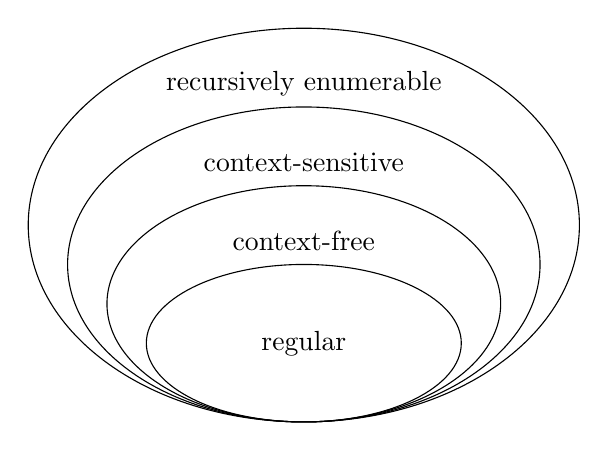
\begin{tikzpicture}
        \draw (0,0) ellipse (2 and 1);
        \draw (0,0.5) ellipse (2.5 and 1.5);
        \draw (0,1) ellipse (3 and 2);
        \draw (0,1.5) ellipse (3.5 and 2.5);
        \node at (0,0) {regular};
        \node at (0,1.3) {context-free};
        \node at (0,2.3) {context-sensitive};
        \node at (0,3.3) {recursively enumerable};
    \end{tikzpicture}
    \caption{Chomsky hierarchy of formal languages}
    \label{fig:chomsky-hierarchy}
\end{figure}

\subsubsection{Practical Implications}
The theoretical constructs discussed above are not only of academic interest but also have significant practical applications:
\begin{itemize}
    \item \textbf{Regular Expressions}: Extensively used in text processing (e.g., in tools such as \texttt{grep} and in lexical analysers) \cite{kernighan1984unix, hopcroft2006introduction}.
    \item \textbf{Context-Free Grammars}: Form the basis for defining the syntax of programming languages such as Python and Java \cite{chomsky1956three, hopcroft2006introduction}.
    \item \textbf{Closure Properties}: Provide a framework for proving decidability results (e.g., the emptiness problem for \glspl{dfa}) \cite{hopcroft2006introduction}.
    \item \textbf{Stochastic Models}: Are applied in areas like natural language processing and speech recognition, where probabilistic pattern matching is essential \cite{rabin1963probabilistic}.
\end{itemize}
\subsection{\glsentrylongpl{cfa} Definition Fundamentals}
\label{subsec:automata-definition-fundamentals}

All automata share several core structural components that provide the basis for their computational behavior \cite{hopcroft2006introduction, sipser2013introduction}.

\begin{definition}[\glsentrylong{cfa}]
\label{def:finite-automaton}
A \textit{finite automaton} is a computational model that processes input symbols to recognise languages. Formally, a finite automaton $M$ is a quintuple $(Q, \Sigma, \delta, q_0, F)$, where:
\begin{itemize}
    \item \textbf{States ($Q$)}: A finite set of configurations representing the progress of computation \cite{sipser2013introduction}.
    \item \textbf{Input Alphabet ($\Sigma$)}: A finite set of symbols that the automaton processes \cite{hopcroft2006introduction, sudkamp2006languages}.
    \item \textbf{Transition Function ($\delta$)}: A function that governs state changes based on input. For deterministic models, $\delta: Q \times \Sigma \to Q$ is a total function (defined for all state-symbol pairs); for nondeterministic models, $\delta: Q \times \Sigma \to 2^Q$ \cite{sipser2013introduction}.
    \item \textbf{Initial State ($q_0 \in Q$)}: The starting configuration of the automaton \cite{hopcroft2006introduction}.
    \item \textbf{Accept States ($F \subseteq Q$)}: A subset of states indicating successful recognition of an input string \cite{sipser2013introduction}.
\end{itemize}
\end{definition}

\begin{remark}
The quintuple $(Q, \Sigma, \delta, q_0, F)$ provides a standardised representation for comparing automata models. The term "total function" in \glspl{dfa} means every state-symbol pair has exactly one transition \cite{sipser2013introduction}.
\end{remark}

\begin{example}
The \gls{dfa} in Figure~\ref{fig:cfa-example} is defined by:
\begin{itemize}
    \item $Q = \{q_0, q_1\}$,
    \item $\Sigma = \{0, 1\}$,
    \item Transitions: $\delta(q_0, 0) = q_0$, $\delta(q_0, 1) = q_1$, $\delta(q_1, 0) = q_1$, $\delta(q_1, 1) = q_0$,
    \item $F = \{q_0\}$, accepting strings with an even number of 1s.
\end{itemize}
\end{example}

\begin{figure}[htbp]
    \centering
    \begin{tikzpicture}[->,>=stealth,shorten >=1pt,auto,node distance=3cm,
                        semithick, every state/.style={minimum size=0.8cm}]
        % States
        \node[state, initial, accepting] (q0) {$q_0$};
        \node[state] (q1) [right=of q0] {$q_1$};
        
        % Transitions
        \path 
            (q0) edge [loop above] node {0} (q0)
                 edge [bend left=20] node {1} (q1)
            (q1) edge [loop above] node {0} (q1)
                 edge [bend left=20] node {1} (q0);
    \end{tikzpicture}
    \caption{\gls{dfa} recognizing strings with an even number of 1s. The double circle indicates the accept state $q_0$.}
    \label{fig:cfa-example}
\end{figure}

\begin{observation}
Graphical representations provide an intuitive understanding of automata behavior \cite{kozen1997automata, sudkamp2006languages}. 
Key conventions include:
\begin{itemize}
    \item \textbf{States}: Circles labeled with state names (e.g., $q_0$).
    \item \textbf{Initial State}: Marked by an unlabeled incoming arrow.
    \item \textbf{Accept States}: Double circles (e.g., $q_0$ in Figure~\ref{fig:cfa-example}).
    \item \textbf{Transitions}: Arrows labeled with input symbols.
\end{itemize}
\end{observation}

\begin{table}[htbp]
    \centering
    \begin{adjustbox}{max width=\textwidth}
      \begin{tabular}{@{}lllll@{}}
          \toprule
          \textbf{Automaton} & \textbf{Memory} & \textbf{Transitions} & \textbf{Acceptance Condition} & \textbf{Reference} \\ \midrule
          \gls{dfa} & None & Deterministic & Final state & \cite{sipser2013introduction} \\
          \gls{nfa} & None & Nondeterministic & Any accepting path & \cite{hopcroft2006introduction} \\
          \gls{pda} & Stack & Nondeterministic & Final state or empty stack & \cite{sipser2013introduction} \\
          \gls{tm} & Infinite tape & Deterministic & Halting in accept state & \cite{turing1936computable} \\
          \bottomrule
      \end{tabular}
    \end{adjustbox}
    \caption{Automata variations: structural and operational differences}
    \label{tab:automata-variations}
\end{table}


\subsection{Deterministic Finite Automata (DFA)}
\label{subsec:dfa} 

A DFA is a quintuple $M = (Q, \Sigma, \delta, q_0, F)$, where:
\begin{itemize}
    \item $Q$: Finite set of states.
    \item $\Sigma$: Input alphabet.
    \item $\delta: Q \times \Sigma \to Q$: Deterministic transition function.
    \item $q_0 \in Q$: Initial state.
    \item $F \subseteq Q$: Accepting states \cite{hopcroft2006introduction}.
\end{itemize} 

Computation proceeds deterministically: for input $w = a_1 a_2 \dots a_n$, the state evolves as $\delta(q_{i-1}, a_i) = q_i$ \cite{hopcroft2006introduction}. A string $w$ is accepted if $\delta(q_0, w) \in F$. DFAs recognize precisely the regular languages, with expressive power strictly weaker than context-free languages \cite{hopcroft2006introduction}. 

Key properties include:
\begin{itemize}
    \item \textit{Minimization}: Hopcroft's algorithm reduces DFAs to minimal form in $O(n \log n)$ time \cite{hopcroft2006introduction}.
    \item \textit{Emptiness Problem}: Decidable via reachability analysis from $q_0$ to $F$ \cite{hopcroft2006introduction}.
    \item \textit{Pumping Lemma}: For any $L \in \text{REG}$, there exists $p$ such that any $w \in L$ with $\|w\| \geq p$ can be decomposed as $w = xyz$ (with $\|xy\| \leq p$, $\|y\| \geq 1$) such that $xy^i z \in L$ for all $i \geq 0$ \cite{hopcroft2006introduction}.
\end{itemize} 

\newpage
\subsection{\acrfull{nfa}}
\label{subsec:nfa}
\begin{definition}[\gls{nfa}]
    A \gls{nfa} is a quintuple 
    \[
    M = (Q, \Sigma, \delta, q_0, F)
    \]
    where:
    \begin{itemize}
        \item \( Q \) is a finite set of states \cite{kozen1997automata},
        \item \( \Sigma \) is an input alphabet \cite{sudkamp2006languages},
        \item \( \delta: Q \times (\Sigma \cup \{\epsilon\}) \rightarrow 2^Q \) is a nondeterministic transition function \cite{hopcroft2006introduction},
        \item \( q_0 \in Q \) is the initial state,
        \item \( F \subseteq Q \) is the set of accepting states.
    \end{itemize}
\end{definition}

\begin{remark}
Unlike \glspl{dfa}, a \gls{nfa} may have multiple transitions for a given state and input symbol, including transitions on the empty string \(\epsilon\). This nondeterminism allows for multiple computational paths.
\end{remark}

\begin{example}
Figure~\ref{fig:nfa-example} depicts a \gls{nfa} that recognises the language 
\[
L = \{ w \in \{a,b\}^* \mid w \text{ contains the substring } ab \}.
\]
\end{example}

\begin{algorithm}[Subset Construction for \glspl{nfa}]
\label{alg:subset}
To convert an \gls{nfa} \( N = (Q, \Sigma, \delta, q_0, F) \) into an equivalent \gls{dfa} \cite{hopcroft2006introduction, kozen1997automata}:
\begin{enumerate}
    \item Compute the \(\epsilon\)-closure of the initial state: \( S_0 = \epsilon\text{-closure}(\{q_0\}) \).
    \item For each \gls{dfa} state \( S \subseteq Q \) and each input symbol \(\sigma \in \Sigma\), define 
    \[
    \delta_{\text{\gls{dfa}}}(S, \sigma) = \epsilon\text{-closure}\Big(\bigcup_{q \in S} \delta(q, \sigma)\Big).
    \]
    \item Mark \( S \) as accepting if \( S \cap F \neq \emptyset \).
    \item Repeat until no new states are produced.
\end{enumerate}
\end{algorithm}

\begin{observation}
    The subset construction algorithm may produce up to \(2^{|Q|}\) states in the worst case, illustrating a potential state explosion when converting an \gls{nfa} to a \gls{dfa} \cite{sipser2013introduction}.
\end{observation}

\begin{figure}[h]
    \centering  
    \begin{tikzpicture}[shorten >=1pt, node distance=2.5cm, on grid, auto]
        \node[state, initial, initial text={}] (q0) {$q_0$};
        \node[state] (q1) [right=of q0] {$q_1$};
        \node[state, accepting] (q2) [right=of q1] {$q_2$};

        \path[->]
        (q0) edge [loop above] node {$a,b$} (q0)
        (q0) edge node {$a$} (q1)
        (q1) edge node {$b$} (q2);
    \end{tikzpicture}
    \caption{NFA recognizing \( L = \Sigma^*ab \)}
    \label{fig:nfa-example}
\end{figure}

\begin{figure}[h]
    \centering  
    \begin{tikzpicture}[shorten >=1pt, node distance=3cm, on grid, auto]
        \node[state, initial, initial text={}] (A) {$\{q_0\}$};
        \node[state] (B) [right=of A] {$\{q_0, q_1\}$};
        \node[state, accepting] (C) [right=of B] {$\{q_0, q_2\}$};

        \path[->]
        (A) edge [loop below] node {$b$} (A)
        (A) edge node {$a$} (B)
        (B) edge [loop below] node {$a$} (B)
        (B) edge node {$b$} (C)
        (C) edge [bend left] node {$a$} (B)
        (C) edge [bend right] node[swap] {$b$} (A);
    \end{tikzpicture}
    \caption{Equivalent DFA for NFA in Figure~\ref{fig:nfa-example} \cite{hopcroft2006introduction}}
    \label{fig:dfa-conversion}
\end{figure}
\subsection{\glsentrylong{pfa}}
\label{subsec:pfa}

\begin{definition}[\glsentrylong{pfa}]
    A \gls{pfa} is a quintuple 
    \[
    M = (Q, \Sigma, \delta, \pi, F)
    \]
    where:
    \begin{itemize}
        \item \( Q \) is a finite set of states,
        \item \( \Sigma \) is a finite input alphabet,
        \item \( \delta: Q \times \Sigma \times Q \rightarrow [0,1] \) is a probabilistic transition function \cite{rabin1963probabilistic} such that 
        \[
        \sum_{q' \in Q} \delta(q, \sigma, q') = 1 \quad \text{for all } q \in Q \text{ and } \sigma \in \Sigma
        ,\]
        \item \( \pi \in \mathbb{R}^{|Q|} \) is an initial state distribution vector with 
        \[
        \sum_{q \in Q} \pi_q = 1,
        \]
        \item \( F \subseteq Q \) is the set of accepting states.
    \end{itemize}
\end{definition}

\begin{remark}
In a \gls{pfa}, transitions are probabilistic. The acceptance of an input string is determined by whether the cumulative probability of ending in an accepting state exceeds a chosen cut-point.
\end{remark}

\begin{example}
Figure~\ref{fig:pfa-example} illustrates a \gls{pfa} that recognises the language 
\[
L_{\text{maj}} = \{ w \in \{a,b\}^* \mid |w|_a > |w|_b \},
\]
where the acceptance probability is at least \( \frac{2}{3} \).
\end{example}

%TODO: Explain the computation of the acceptance probability
\begin{figure}[ht]
    \centering  
    \begin{tikzpicture}[shorten >=1pt, node distance=3cm, on grid, auto]
        \node[state, initial, initial text={$\pi=1$}] (q0) {$q_0$};
        \node[state, accepting] (q1) [right=of q0] {$q_1$};
        
        \path[->]
        (q0) edge [loop above] node {a(0.6), b(0.4)} (q0)
        (q0) edge [bend left] node {a(0.4), b(0.6)} (q1)
        (q1) edge [loop above] node {a(0.3), b(0.7)} (q1)
        (q1) edge [bend left] node {a(0.7), b(0.3)} (q0);
    \end{tikzpicture}
    \caption{PFA for majority language with probabilistic transitions}
    \label{fig:pfa-example}
\end{figure}

\begin{theorem}[Rabin's Theorem for \glspl{pfa}]
    \label{thm:rabin}
    A \gls{pfa} with an isolated cut-point recognises exactly the class of regular languages \cite{rabin1963probabilistic}.
\end{theorem}

\begin{proposition}
    If a \gls{pfa} employs a non-isolated cut-point (e.g., \(\lambda = 0\)), it may recognise languages beyond the regular class, including some context-sensitive languages \cite{paz1971introduction}.
\end{proposition}

\begin{corollary}
For a \gls{pfa} with a strict cut-point (\(\lambda = 1\)), the recognised language is equivalent to that of a \gls{dfa}.
\end{corollary}

\begin{observation}
    The closure properties of \glspl{pfa} differ from those of classical finite automata. In particular, complementation is not directly achievable unless an isolated cut-point is used \cite{droste2009handbook}.
\end{observation}

\subsection{Two-Way Finite Automata Variants}
\label{subsec:two-way-variants}

Two-way finite automata extend the classical one‐way model by allowing the read head to move in both directions over the input. Although this extra power does not increase the class of recognizable languages, two-way models can be exponentially more succinct than one-way models \cite{sakoda1978nfas, kozen1997automata} and naturally lend themselves to algorithms in several contexts (e.g., in complexity analysis and even quantum models).

\subsubsection{\glsentrylong{2dfa}}
\label{subsubsec:2dfa}

\begin{definition}[\glsentrylong{2dfa}]
A \gls{2dfa} is formally defined as an 8-tuple 
\[
M = (Q, \Sigma, \triangleright, \dashv, \delta, s, t, r),
\]
where:
\begin{itemize}
  \item \(Q\) is a finite set of states,
  \item \(\Sigma\) is a finite input alphabet,
  \item \(\triangleright\) and \(\dashv\) are special symbols called the left and right endmarkers, respectively (with \(\triangleright,\dashv \notin \Sigma\)),
  \item \(\delta: Q \times (\Sigma \cup \{\triangleright, \dashv\}) \to Q \times \{\triangleright,\dashv\}\) is the transition function,
  \item \(s\in Q\) is the start state,
  \item \(t\in Q\) is the unique accept state,
  \item \(r\in Q\) (with \(r\neq t\)) is the unique reject state.
\end{itemize}
In addition, the transition function is assumed to satisfy:
\begin{itemize}
  \item For every state \(q\in Q\), when reading the left endmarker \(\triangleright\), the head always moves in the \(\dashv\) direction; that is, \(\delta(q,\triangleright) = (q', \dashv)\) for some \(q'\in Q\).
  \item Similarly, when reading the right endmarker \(\dashv\), the head always moves in the \(\triangleright\) direction: \(\delta(q,\dashv) = (q', \triangleright)\).
  \item Once the machine reaches the accept state \(t\) (or the reject state \(r\)), it remains there (the transition always maps back to itself) while moving in a fixed direction.
\end{itemize}
\end{definition}

\begin{remark}
The two-way motion allows the automaton to perform multiple passes over the input, which can result in an exponential reduction in the number of states compared to one-way automata, though at the expense of increased operational complexity.
\end{remark}

\begin{example}
    Consider the language 
    \[
    L = \{ w\in \{0,1\}^* \mid \text{the first symbol of } w \text{ equals the last symbol} \}.
    \]
    A \gls{2dfa} for \(L\) operates as follows:
    \begin{enumerate}
      \item Start at \(\triangleright\) and move in the \(\dashv\) direction to read the first symbol, transitioning to a state encoding this symbol (e.g., \(q_a\) for \(a \in \{0,1\}\)).
      \item Continue moving in the \(\dashv\) direction until \(\dashv\) is reached.
      \item Reverse direction and scan in the \(\triangleright\) direction to the last symbol.
      \item Compare the stored symbol (encoded in the current state) with the last symbol. Accept if they match; reject otherwise.
    \end{enumerate}
\end{example}

\begin{observation}
    Although every \gls{2dfa} can be simulated by a \gls{1dfa}, such a simulation may require an exponential increase in the number of states \cite{shepherdson1959reduction}.
\end{observation}

\paragraph{Operational Mechanics}
The two-way motion enables the automaton to make multiple passes over the input, which is particularly useful for verifying properties that depend on both the prefix and the suffix of the input string.

\paragraph{State Complexity and Conversion Algorithms}
For some families of regular languages, \glspl{2dfa} can be exponentially more succinct than their one-way counterparts. Conversion algorithms—such as those proposed by Shepherdson and Kozen—use crossing sequences to simulate two-way behavior in a one-way \gls{dfa}, typically at the cost of exponential state blow-up.

%TODO: enhance the following example
\begin{figure}[ht]
    \centering  
    \begin{tikzpicture}[shorten >=1pt, node distance=2.5cm, on grid, auto]
        \node[state,initial,accepting] (q0) {\(q_0\)};
        \node[state] (q1) [right=of q0] {\(q_1\)};
        \node[state] (q2) [below=of q1] {\(q_2\)};
        \node[state,accepting] (t) [left=of q2] {\(t\)};
        \node[state,rejecting] (r) [right=of q2] {\(r\)};

        \path[->]
            (q0) edge node[above] {\(\triangleright \to \dashv,\, \text{store } a\)} (q1)
            (q1) edge [loop above] node {\(\sigma,\dashv\)} (q1)
            (q1) edge node[right] {\(\dashv \to \triangleright\)} (q2)
            (q2) edge [loop below] node {\(\sigma,\triangleright\)} (q2)
            (q2) edge node[below] {\(\triangleright: a = \text{last?}\)} (t)
            (q2) edge node[above] {\(\triangleright: a \neq \text{last}\)} (r);
    \end{tikzpicture}
    \caption{\gls{2dfa} for \(L = \{w \mid w_1 = w_{|w|}\}\). States encode the first symbol \(a \in \{0,1\}\). Transitions use \(\triangleright/\dashv\) to denote head movement directions and endmarkers.}
    \label{fig:2dfa-example}
\end{figure}

\subsubsection{\glsentrylong{2nfa}}
\label{subsubsec:2nfa}

\begin{definition}[\glsentrylong{2nfa}]
A \gls{2nfa} is defined similarly to a \gls{2dfa} but with a nondeterministic transition function \cite{sakoda1978nfas}. Formally, a \gls{2nfa} is an 8-tuple
\[
M = (Q, \Sigma, \triangleright, \dashv, \delta, s, t, r),
\]
where:
\begin{itemize}
    \item \(Q\) is a finite set of states,
    \item \(\Sigma\) is a finite input alphabet,
    \item \(\triangleright\) and \(\dashv\) are the left and right endmarkers (with \(\triangleright,\dashv \notin \Sigma\)),
    \item \(\delta: Q \times (\Sigma \cup \{\triangleright,\dashv\}) \to 2^{\,Q \times \{\triangleright,\dashv\}}\) is the nondeterministic transition function,
    \item \(s\in Q\) is the start state,
    \item \(t\in Q\) is the unique accept state, and
    \item \(r\in Q\) (with \(r\neq t\)) is the unique reject state.
\end{itemize}
The transition function obeys similar boundary conditions as in the \gls{2dfa} case.
\end{definition}

\begin{remark}
The nondeterminism in a \gls{2nfa} allows it to “guess” important positions within the input and verify them via bidirectional traversal, which can lead to significant state savings compared to deterministic models.
\end{remark}

\begin{example}
Consider the language 
\[
L_{sym} = \{ w \in \{0,1\}^* \mid \text{the first two symbols equal the last two symbols} \}.
\]
A high-level description of a \gls{2nfa} for \(L_{sym}\) is:
\begin{enumerate}
    \item Scan in the \(\dashv\) direction from the left endmarker \(\triangleright\) while nondeterministically guessing the point where comparison will occur.
    \item Upon reaching the right endmarker \(\dashv\), reverse direction.
    \item While moving in the \(\triangleright\) direction, nondeterministically check that the stored first two symbols match the corresponding symbols at the end.
    \item If both comparisons succeed, transition to the accept state \(t\); otherwise, transition to the reject state \(r\).
\end{enumerate}
Figure~\ref{fig:2nfa-example} schematically illustrates this guess-and-check mechanism.
\end{example}

%TODO: enhance the following example
\begin{figure}[ht]
    \centering  
    \begin{tikzpicture}[shorten >=1pt, node distance=2.2cm, on grid, auto]
        \node[state,initial] (q0) {\(q_0\)};
        \node[state] (q1) [right=of q0] {\(q_1\)};
        \node[state] (q2) [right=of q1] {\(q_2\)};
        \node[state,accepting] (qa) [above=of q2] {\(t\)};
        \node[state,rejecting] (qr) [below=of q2] {\(r\)};
        
        \path[->]
            (q0) edge [loop above] node {\(\sigma,\dashv\)} (q0)
            (q0) edge node {\(\triangleright \to \dashv\)} (q1)
            (q1) edge [loop above] node {\(\sigma,\dashv\)} (q1)
            (q1) edge node {\(\dashv \to \triangleright\)} (q2)
            (q2) edge [bend left] node[above left] {\(\sigma,\triangleright\) (guess)} (q0)
            (q2) edge node[right] {\(\sigma = \text{stored?}\)} (qa)
            (q2) edge node[right] {\(\sigma \neq \text{stored}\)} (qr);
    \end{tikzpicture}
    \caption{2NFA for \(L_{\text{sym}} = \{ww^R\}\). The machine nondeterministically guesses the midpoint (via transition \(q_2 \to q_0\)) and verifies symmetry.}
    \label{fig:2nfa-example}
\end{figure}

\begin{observation}
\glspl{2nfa} can be exponentially more succinct than one-way \glspl{dfa}, even though the class of languages they recognise remains the same (i.e., the regular languages).
\end{observation}

\subsubsection{\glsentrylong{2pfa}}
\label{subsubsec:2pfa}

\begin{definition}[\glsentrylong{2pfa}]
A \gls{2pfa} is an 8-tuple
\[
M = (Q, \Sigma, \triangleright, \dashv, \delta, s, t, r),
\]
where:
\begin{itemize}
    \item \(Q\) is a finite set of states,
    \item \(\Sigma\) is a finite input alphabet,
    \item \(\triangleright\) and \(\dashv\) are the left and right endmarkers (with \(\triangleright,\dashv \notin \Sigma\)),
    \item \(\delta: Q \times (\Sigma \cup \{\triangleright,\dashv\}) \to \mathbb{R}_{\ge 0}^{\,Q \times \{\triangleright,\dashv\}}\) is a probabilistic transition function such that
    \[
    \sum_{(q',d)\in Q\times\{\triangleright,\dashv\}} \delta(q,a,q',d) = 1 \quad \text{for all } q \in Q \text{ and } a \in \Sigma \cup \{\triangleright,\dashv\},
    \]
    \item \(s\in Q\) is the start state,
    \item \(t\in Q\) is the unique accept state, and
    \item \(r\in Q\) (with \(r\neq t\)) is the unique reject state.
\end{itemize}
\end{definition}

\begin{remark}
A \gls{2pfa} extends the probabilistic finite automaton by allowing bidirectional head movement. Its transitions are governed by probability distributions, and acceptance is determined by whether the cumulative probability of reaching the accept state exceeds a predetermined cut-point.
\end{remark}

%TODO: link to the previous example, cardinality symbol now is different
\begin{example}
Consider the language 
\[
L_{maj} = \{ w \in \{a,b\}^* \mid \#a(w) > \#b(w) \}.
\]
A \gls{2pfa} for \(L_{maj}\) operates by making probabilistic passes over the input, updating state probabilities, and eventually halting in the accept state \(t\) if the acceptance probability is high enough. Figure~\ref{fig:2pfa-example} provides a schematic illustration of such a machine.
\end{example}

\begin{figure}[ht]
    \centering  
    \begin{tikzpicture}[shorten >=1pt, node distance=2.5cm, on grid, auto]
        \node[state,initial] (q0) {\(q_0\)};
        \node[state] (q1) [right=of q0] {\(q_1\)};
        \node[state,accepting] (q2) [right=of q1] {\(t\)};
        \node[state,rejecting] (qr) [below=of q1] {\(r\)};
        
        \path[->]
            (q0) edge [loop above] node[align=center] 
                {\(a:0.6,\dashv\)\\\(b:0.4,\dashv\)} (q0)
            (q0) edge node[above] {\(\dashv \to \triangleright\)} (q1)
            (q1) edge [loop above] node[align=center] 
                {\(a:0.7,\triangleright\)\\\(b:0.3,\triangleright\)} (q1)
            (q1) edge node[above] {\(\triangleright: \Pr(\text{accept}) \geq 2/3\)} (q2)
            (q1) edge node[below left] {\(\triangleright: \Pr(\text{reject}) \geq 1/3\)} (qr);
    \end{tikzpicture}
    \caption{2PFA for \(L_{\text{maj}} = \{w \mid \#a(w) > \#b(w)\}\). Transitions use probabilistic counts with isolated cut-point \(\lambda = 2/3\), and head movements are indicated by \(\triangleright\) (leftward) and \(\dashv\) (rightward).}
    \label{fig:2pfa-example}
\end{figure}

\begin{theorem}[Dwork-Stockmeyer Theorem]
    \label{thm:2pfa-rabin}
    A \gls{2pfa} with an isolated cut-point recognises exactly the class of regular languages \cite{dwork1990time}.
\end{theorem}

\begin{proposition}
If a \gls{2pfa} employs a non-isolated cut-point (e.g., \(\lambda = 0\)), it may recognise languages beyond the regular class.
\end{proposition}

%TODO: add these explainations to the 1PFA too.
\begin{corollary}
For a \gls{2pfa} with a strict cut-point (\(\lambda = 1\)), the recognised language is equivalent to that of a \gls{dfa}.
\end{corollary}

\subsubsection{Comparative Analysis of Two-Way Models}
\label{subsubsec:two-way-comparison}

%TODO: check the correctness of the following table and specify 2PFA. Moreover, add comparison summary also for 1 way models.

\begin{table}[ht]
    \label{tab:two-way-comparison}
    \centering
    \begin{tabular}{|l|c|c|c|c|l|}
        \hline
        \textbf{Model} & \textbf{Language Class} & \textbf{Time} & \textbf{Space} & \textbf{States} & \textbf{Key Reference} \\ 
        \hline
        \gls{2dfa}  & REG & \(O(n^2)\) & \(O(1)\) & \(2^{\Theta(n)}\) & \cite{shepherdson1959reduction} \\
        \gls{2nfa}  & REG & \(O(n)\) & \(O(1)\) & \(O(1)\) & \cite{sakoda1978nfas} \\
        \gls{2pfa}  & REG (isolated cut) & \(O(n^3)\) & \(O(\log n)\) & \(O(1)\) & \cite{dwork1990time} \\
        \hline
    \end{tabular}
    \caption{Comparative analysis of two-way automata models}
\end{table}

\begin{remark}
The comparative analysis illustrates that while all two-way automata recognise only regular languages, the two-way models often achieve significant advantages in state complexity and, in some cases, time complexity, compared to their one-way counterparts.
\end{remark} 
